%
% Hello! Here's how this works:
%
% You edit the source code here on the left, and the preview on the
% right shows you the result within a few seconds.
%
% Bookmark this page and share the URL with your co-authors. They can
% edit at the same time!
%
% You can upload figures, bibliographies, custom classes and
% styles using the files menu.
%
% If you're new to LaTeX, the wikibook at
% http://en.wikibooks.org/wiki/LaTeX
% is a great place to start, and there are some examples in this
% document, too.
%
% Enjoy!
%
\documentclass[12pt,a4paper]{article}

\usepackage[german]{babel}
\usepackage[utf8x]{inputenc}
\usepackage{amsmath}
\usepackage{enumitem}
\usepackage{graphicx}
\usepackage{fancyhdr}
\usepackage{longtable}
\usepackage{lastpage}
\usepackage[bottom]{footmisc}
\usepackage{listings}
\usepackage{rotating}
\usepackage{changepage}   % for the adjustwidth environment
\usepackage[cm]{fullpage}
\usepackage[parfill]{parskip}
\usepackage[table]{xcolor}

\title{Anwenderdokumentation VHDL}
\author{Amar Saljic, Arseniy Vershinin, Jonathan Kienzle}
\date{12. Juli 2013}

\pagestyle{fancy}
\fancyhead{} % clear all header fields
\fancyhead[RE,LO]{\emph{Anwenderdokumentation VHDL - Gruppe 50}}
\renewcommand{\headrulewidth}{0pt} % no line in header area
\fancyfoot{} % clear all footer fields
\fancyfoot[LE,RO]{\thepage /\pageref{LastPage}}           % page number in "outer" position of footer line
%\fancyfoot[RE,LO]{\emph{Anwenderdokumentation VHDL - Gruppe 50}} % other info in "inner" position of footer line

\begin{document}
\definecolor{lightgray}{gray}{0.9}
\maketitle

\thispagestyle{fancy}

\section{Übersicht}

Die getaktete Ablaufsteuerung (Timing Generator) ist Teil eines S/PDIF Konverters, welcher zusätzlich aus einem Data-Multiplexer, Biphase-Mark Encoder und Subcode Generator besteht. Der Timing Generator stimmt dabei die Generierung von Frames, Subframes, Präambeln und Subcodedaten zeitlich ab, indem er entsprechende Signale an die beteiligten Bausteine ausgibt.\newline Die Daten werden in Blöcke von 192 Frames aufgeteilt, die jeweils aus zwei Subframes bestehen, welche unter anderem die Daten für den linken bzw. rechten Audiokanal enthalten. Der genaue Aufbau eines Subframes wird in folgender Grafik dargestellt:
\vspace{0.4cm}

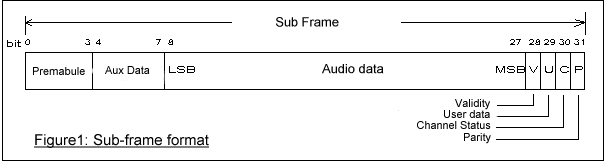
\includegraphics[width=18cm]{_fig1.png}\newline
\section{Blackbox-Beschreibung}
Der Timing Generator verfügt über die folgenden 1 Bit Ein- und Ausgänge: \newline \newline
Eingänge:
\begin{itemize}
\item {\bf CLK:} Taktsignaleingang, dessen Frequenz die verdoppelte Frequenz der eigentlichen Bitrate ist (bei 44kHz Samplerate wird auf 5,6MHz getaktet).
\item {\bf RESET:} sorgt dafür, dass alle Signale auf ihren Startwert zurückgesetzt werden.
\end {itemize}
\noindent

Ausgänge:
\begin {itemize}
\item {\bf SHIFTCLK:} legt fest, ob der Shiftregister des Data-Multiplexers die eingehende Daten verschieben soll.
\item {\bf LOAD\_L\textbackslash LOAD\_R:} legt fest, ob die Daten des linken oder rechten Kanals mit Hilfe des Data-Multiplexers an den Biphase-Mark Encoder weitergeleitet werden solle
\item {\bf START:} legt fest, ob der Subcode Generator die User Data, Channel Status oder Validity Bits ausgeben soll.
\item {\bf X\textbackslash Y:} legt fest, ob der Biphase-Mark Encoder eine Präambel für den linken (X) bzw. rechten (Y) Kanal kodieren und ausgeben soll.
\item {\bf Z:} legt fest, ob der Biphase-Mark Encoder eine Präambel für den Anfang eines Blocks kodieren und ausgeben soll.
\item {\bf P:} legt fest, ob der Biphase-Mark Encoder ein Parity-Bit ausgegeben soll.
\end{itemize}
\subsection*{Anmerkung}
Es wird davon ausgegangen, dass der vom Timing Generator gesteuerte Data-Multiplexer mit \newline 16-bitigen Samples arbeitet.
\section{Beispielszenario}
\emph{Ziel}: Zeitliche Steuerung der beteiligten Bausteine (Data-Multiplexer, Biphase-Mark Encoder und Subcode Generator).

\emph{Schritte}:
\begin{enumerate}
\item Kontinuierliches Taktsignal (bei 44kHz Samplerate wird auf 5,6MHz getaktet) auf den \emph{CLK}-Eingang legen.
\item \emph{RESET}-Eingang auf '1' setzen.
\item \emph{RESET}-Eingang auf '0' setzen.
\end{enumerate}

\emph{Ergebnis}: Solange ein Taktsignal auf dem \emph{CLK}-Eingang liegt, werden die korrekten Ausgangssignale für die beteiligten Bausteine generiert.

\end{document}